\documentclass[12pt,a4paper]{report}
% importation des packages
\usepackage[utf8]{inputenc}
\usepackage[francais]{babel}
\usepackage{graphicx}
\graphicspath{ {./images/} }
\usepackage{subcaption}
\usepackage{wrapfig}


%hauts et bas de pages
\usepackage{fancyhdr}
\usepackage{color}
\usepackage[dvipsnames]{xcolor}
\usepackage[Glenn]{fncychap}
\pagestyle{fancy}
\lhead{Projet de Science des données}
\rhead{Groupe SantEconomie} 
\lfoot{License MIASHS}
\rfoot{2022/2023} 
\cfoot{\textbf{Page \thepage}}
\renewcommand{\headrulewidth}{1pt}
\renewcommand{\footrulewidth}{1pt}

% Définition du format pour le chapitre pour le mettre en couleur à modifier 
% \titleformat{\chapter}[display]
  % {\normalfont\Large\bfseries\color{myblue}}
  % {\chaptertitlename\ \thechapter}{20pt}{\Huge}

\begin{document}
%------------------------------------------------premiere page
\begin{titlepage}

%logo paul valéry et logo projet
\begin{center}
\begin{figure}[h]
    \centering
    \begin{subfigure}{0.3\textwidth}
        \centering
        
\includegraphics[width=\linewidth]{images/Logo_univ.png}
    \end{subfigure}
    \hspace{3cm}
    \begin{subfigure}{0.4\textwidth}
        \centering
        
\includegraphics[width=\linewidth]{images/Logo_SanEconomie.png}
    \end{subfigure}
    \label{fig:images}
\end{figure}

\medskip
{\Large{Universit\'{e} Paul Val\'{e}ry }}\\
\textsc{UFR 6}\\
 \vskip0.5cm
  \noindent {\textsc{\LARGE \textcolor{MidnightBlue}{Licence MIASHS}}\\[1cm]}
\end{center}
\vskip0.5cm
\begin{center}
\textbf{Projet de science des donn\'{e}es}\\
\vskip0.5cm
%------------------------------------------------
\newcommand{\HRule}{\rule{\linewidth}{0.5mm}} 
	\HRule\\[0.2cm]
	{\huge\bfseries\textcolor{MidnightBlue}{Projet SantEconomie\\[0.2cm]}}
	\HRule\\[1cm]
%------------------------------------------------
Par: \\
\small \bf{\ Girondin Audric, Can Arisoy Ivan, Duckes Jonathan, \\ Carot-Gelas Axel, Ravalisaona Malala, Abdallah Rachydah}
\end{center}
%------------------------------------------------
  \vspace{3mm}
  \centerline {\small \bf{\ Soutenue le $03/05/2022$}}
  \vspace{3mm}
  \centerline {\small \bf{\ Encadrants : $Sandra Bringay, Namrata Patel$}} 
%------------------------------------------------
\vskip2.5cm
\begin{center}
{\small{Année Universitaire : \textbf{2022-2023}}} \\
\end{center}

\end{titlepage}
%------------------------------------------------fin premiere page

% Insertion de la table de matieres
\vspace{-2cm}
\tableofcontents % insertion de table des matières
    
% Introduction Générale
\chapter{Introduction}
\vspace{-1.5cm}
\section{Contexte du projet}
\begin{wrapfigure}[5]{r}{0.3\textwidth}
    \vspace{-2.5em} % ajuster l'espace vertical entre l'image et le texte
    
\includegraphics[width=0.25\textwidth]{images/image_cahier_charge.png}
\end{wrapfigure}
Ce module a pour objectif de nous apprendre à mener à bien un projet de groupe, de sa conception à sa livraison. La conception du projet s'est étalée sur deux semestres :

\begin{itemize}
\item Le premier axé sur la rédaction d'un cahier des charges.
\item Le second sur la réalisation du produit.
\end{itemize}

\section{Enjeux}
Vous êtes un journaliste et vous devez rédiger un article sur le thème de la santé ou de l'économie mondiale ? Vous souhaitez changer de pays et vos critères de sélection comportent la santé et l'économie ? Vous souhaitez tout simplement vous informer sur ces sujets par curiosité ? \\

Nous sommes fiers de vous présenter notre solution utilisant des données précises sur l'économie et la santé de chaque pays entre 1990 et 2021, et nous sommes convaincus que vous trouverez notre site web utile. \\

Voici quelques liens pour avoir un aperçu du projet :

\begin{itemize}
\item Lien de la vidéo de démonstration pour l'utilisation de notre site web et ses fonctionnalités : https://youtu.be/G9LkBv6KOlk
\item Lien de la vidéo de soutenance : https://youtu.be/3RIUgsEaz0g
\item Lien du dépôt GitHub : https://github.com/Axel667/ProjetSante \\
\end{itemize}

Notre site a pour but de renseigner quiconque le souhaite, sur les données reliant la santé et l'économie de chaque pays. Pour cela, nous disposons de données concernant les facteurs suivants :

\begin{itemize}
\item Le PIB par habitant
\item L'espérance de vie
\item Les dépenses en santé
\item Le taux d'obésité \\
\end{itemize}

En somme, notre site web est un outil indispensable pour toute personne qui souhaite comprendre les tendances économiques et de santé mondiales.

\section{Périmètre du projet}
    Notre première vision du projet était de réaliser un site pour permettre aux utilisateurs de consulter les résultats de nos démarches statistiques grâce à différentes visualisations et une map interactive. Ce site devait être uniquement informatif. \\

    Cependant, nous avons décidé d'inclure d'autres fonctionnalités comme :
\begin{itemize}
    \item La création d’article
    \item La création d’un compte 
    \item Le profil administrateur \\
\end{itemize}
    
    Ces fonctionnalités permettent à notre site web de se démarquer des autres sources d'information déjà existantes. 

\chapter{Description technique}
\vspace{-1.5cm}
\section{Technologies utilisées}
Pour la réalisation de notre projet nous avons utilisé :
\begin{itemize}
    \item \textbf{Microsoft Excel, python} avec pandas pour traiter nos données
    \item \textbf{MAMP/WAMP} pour lancer le serveur web local sur nos machines
    \item \textbf{MYSQL} pour effectuer nos requêtes sur la base de données
    \item \textbf{AWS} pour l'hébergement de base de données 
    \item \textbf{Figma} pour réaliser les maquettes de notre site
    \item \textbf{Github, Git, Gitbash} pour collaborer durant le processus de réalisation
    \item \textbf{HTML, PHP} pour la création de nos pages web
    \item \textbf{CSS, tailwind} pour ajouter un style aux différentes pages
    \item \textbf{Chart.js} pour nos graphiques
    \item \textbf{Mapbox GL JS} librairie open-source permettant d'intégrer des cartes 
    \item \textbf{VS code} pour éditer notre code
\end{itemize}
    \begin{center}
        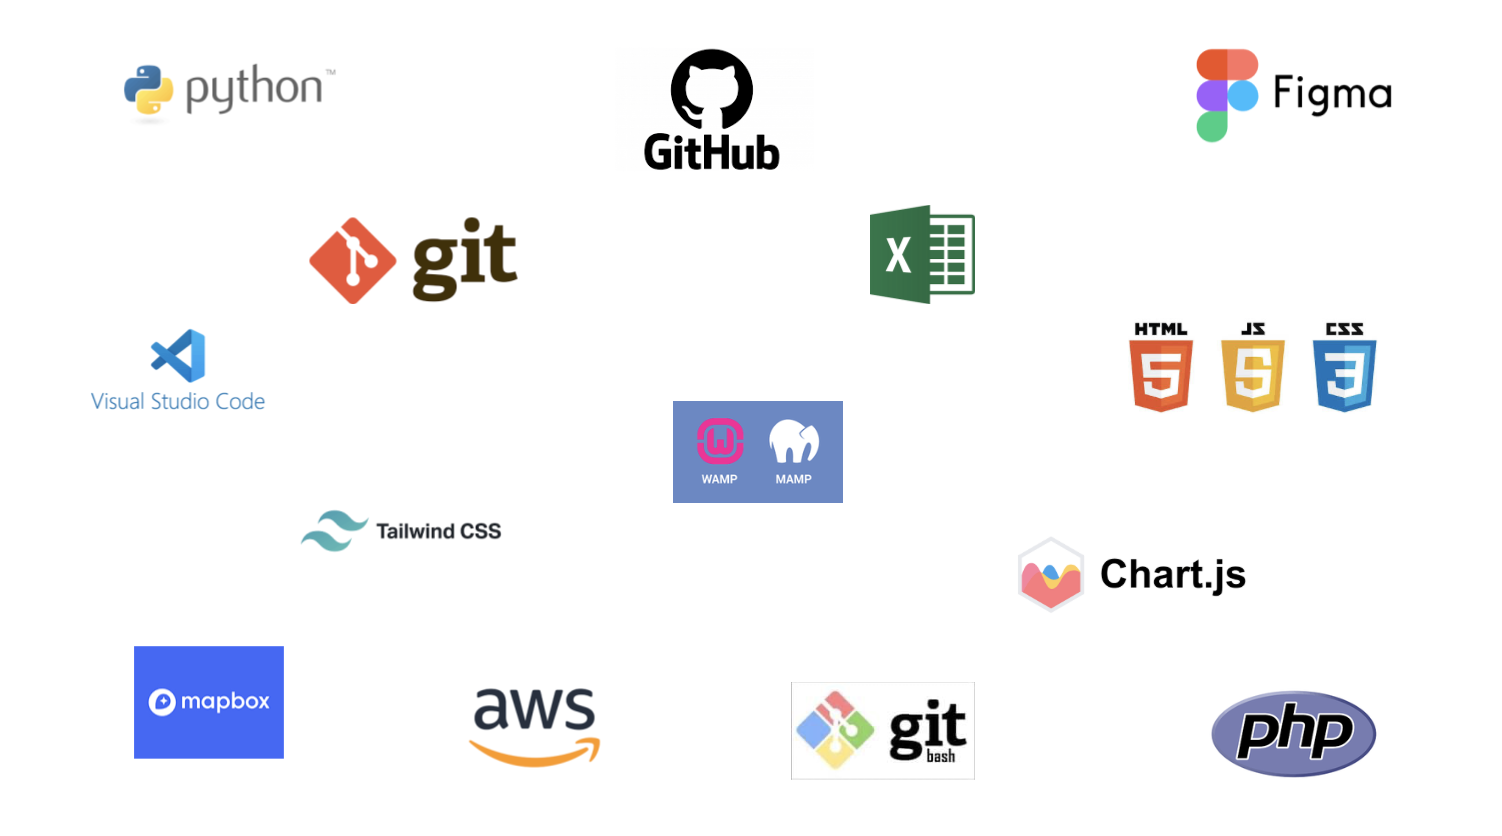
\includegraphics[width=0.9\textwidth]{images/technologies.png}
    \end{center}

\section{Planning}
    \begin{center}
        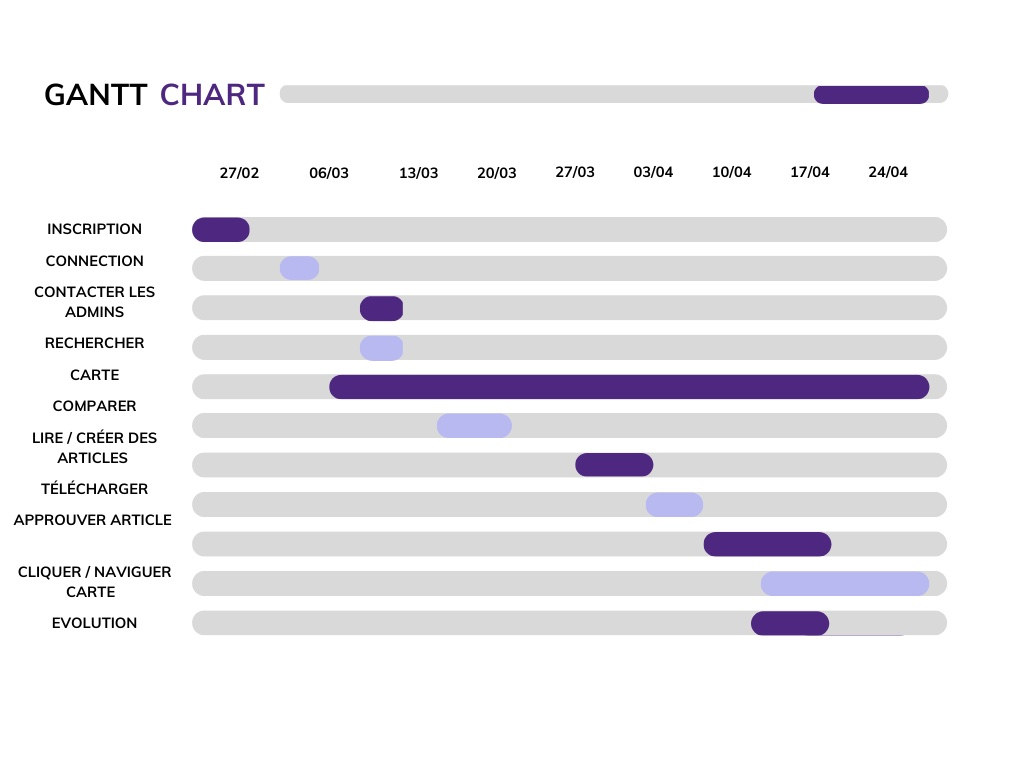
\includegraphics[width=1\textwidth]{images/gantt.jpg}
    \end{center}

    On peut remarquer que la carte est l'étape qui a pris le plus de temps car nous avions des difficultés à afficher les données sur la carte sous forme de pop-up. Cependant, cela ne nous a pas empêché d'avancer sur les autres tâches.
\vspace{0.5cm}
\section{Pré-traitements du jeu de données}
\vspace{0.5cm}

  Au premier semestre, nous avons dû réaliser le prétraitement de notre jeu de données. Pour ce faire, nous avons supprimé les colonnes "population" et "continent" pour les trois premiers fichiers CSV, car nous n'en avons pas besoin dans notre modèle. Nous avons également retiré les valeurs nulles à l'aide des filtres Excel, supprimant ainsi les années où les informations étaient manquantes. \\
  
  Ensuite, nous avons fusionné tous nos fichiers en utilisant la bibliothèque pandas de Python. Plus précisément, nous avons utilisé la fonction merge pour fusionner plusieurs fichiers CSV/DataFrames en nous appuyant sur les colonnes identiques contenant les mêmes informations. Dans notre cas, il s'agissait des colonnes "Entity", "Code" et "Year" pour toutes les informations de la même année. \\

    Nous avons ainsi regroupé toutes nos données dans un seul fichier : "data$\_$csv", afin d'obtenir notre CSV final que nous avons ensuite importé dans SQL.
    
\section{Modèle de la base de donnée (MCD, MOD)}
\subsection{MCD}
    \begin{center}
        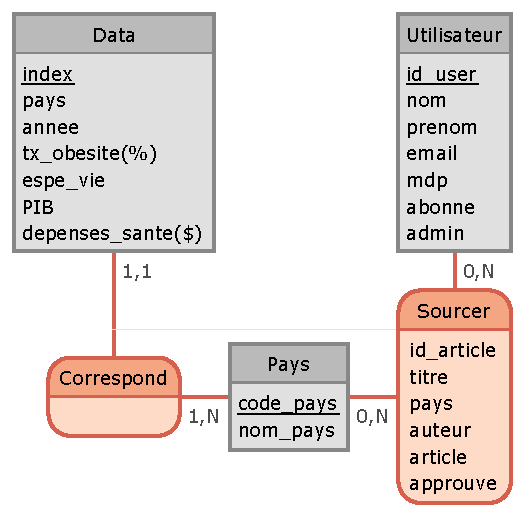
\includegraphics[width=0.5\textwidth]{images/Pays-2.pdf}
    \end{center}
\subsection{MOD}
    \begin{center}
        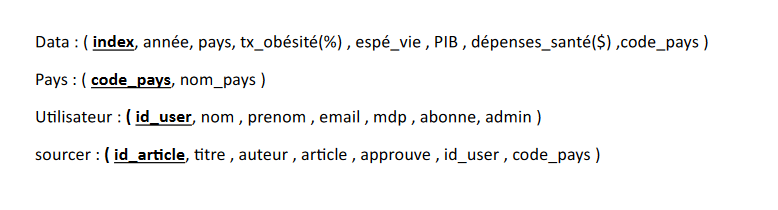
\includegraphics[width=1.1\textwidth]{images/mod.png}
    \end{center}

\section{Schéma de l'architecture}
    \begin{center}
        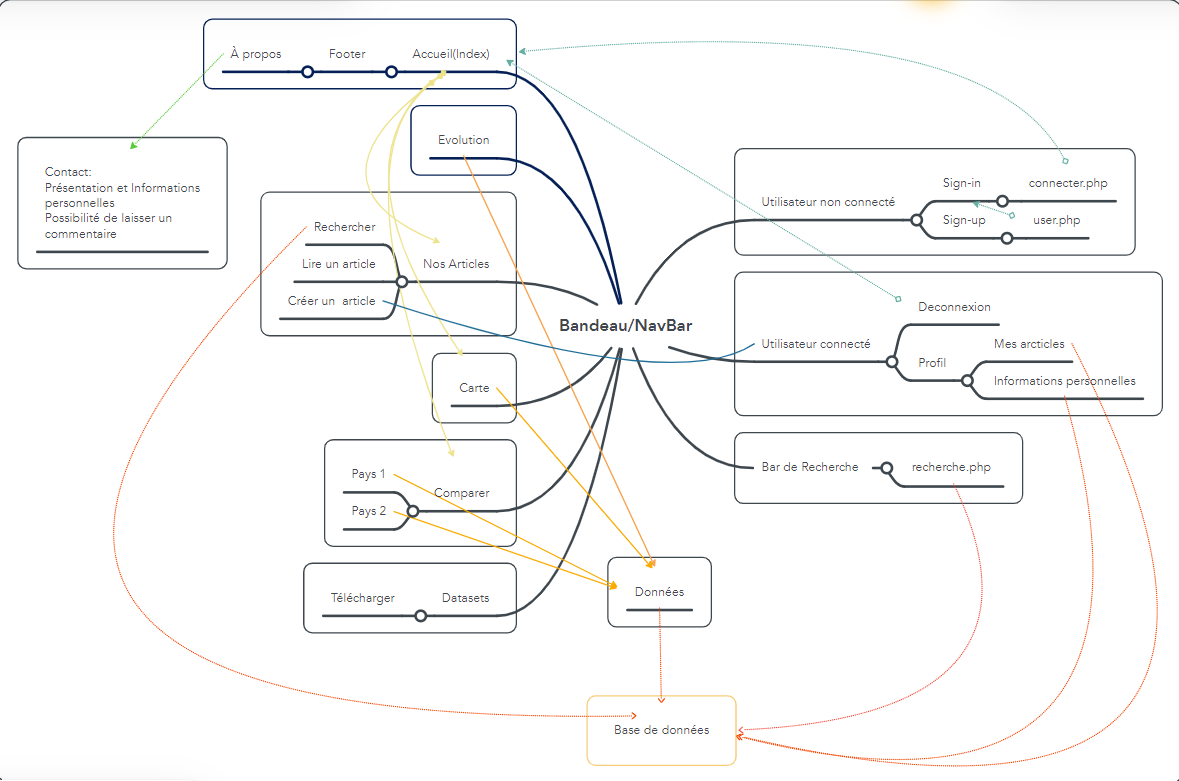
\includegraphics[width=1\textwidth]{images/architecture.png}
        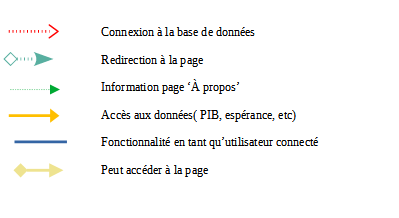
\includegraphics[width=0.5\textwidth]{images/legende_architecture.png}
    \end{center}

\chapter{Description fonctionnelle}
\vspace{-2cm}
\section{L'accueil}
L'utilisateur arrive directement sur la page d'accueil de notre site, où il peut voir, comme sur toutes les autres pages, la barre de navigation qui lui permet de consulter les autres fonctionnalités de notre site.

\section{La carte}
Pour accéder à la carte, il vous est d'abord demandé de sélectionner une année et un type de données. La page génère ensuite un globe terrestre avec lequel vous pouvez naviguer et consulter les données de chaque pays en cliquant sur celui-ci. Une légende avec des couleurs permet une meilleure compréhension de la carte.

\section{Comparer}
Notre site vous permet de comparer ou non les pays au cours du temps en sélectionnant le type de données et de graphique que vous souhaitez.

\section{Évolution}
Il est possible de consulter l'évolution du PIB d'un pays en fonction des autres indicateurs en sélectionnant le type de graphique.

\section{Nos articles}
La page "Articles" vous permet de consulter une liste des articles approuvés par l'administrateur et postés par les utilisateurs ayant un compte. Une barre de recherche vous permet de trouver plus facilement les articles qui font référence à un pays spécifique. Lorsque vous cliquez sur un article, vous êtes redirigé vers une page dédiée affichant le contenu de celui-ci. L'administrateur peut également, lorsqu'il est connecté, approuver ou désapprouver les articles rédigés par les utilisateurs et décider de les rendre visibles ou non.

\section{Datasets}
Nous mettons à disposition les données utilisées par notre site en offrant la possibilité de les télécharger sous différents formats (SQL, CSV, XLSX, JSON).

\section{Barre de recherche}
Cette barre de recherche permet d'obtenir rapidement toutes les données que nous possédons sur un pays.

\section{Sign-up}
Cette fonctionnalité permet aux utilisateurs de créer leur compte sur notre site.

\section{Sign-in}
Cette fonctionnalité permet aux utilisateurs de se connecter à leur compte préalablement créé sur notre site.

\section{Page profil}
Une fois connecté, l'utilisateur peut avoir accès à sa page de profil répertoriant les informations renseignées lors de la création du compte ainsi que ses articles créés et leur statut (approuvé, désapprouvé ou en cours de vérification).

\section{Log out}
Une fois connecté, l'utilisateur peut également se déconnecter de son compte utilisateur.

\section{Créer un article}
Cette possibilité apparaît dans le bandeau uniquement lorsque l'utilisateur est connecté à son compte utilisateur. Pour créer un article, il faut mettre un titre, un nom d'auteur, sélectionner un pays concerné par l'article, le rédiger dans la partie "Article" puis l'enregistrer.

\section{À propos}
Cette page est visible en bas de la page d'accueil où il y est inscrit une courte présentation du projet, une liste des membres du groupe ainsi que leurs adresses email étudiantes.

\chapter{Conclusion}
\section{Tableau des tâches}
\vspace{0.4cm}
\begin{tabular}{|c|c|c|c|c|c|c|}
\hline
Tâches & Audric & Malala & John & Axel & Ivan & Rachydah \\
\hline
MCD/MOD & 16\% & 16\% & 16\% & 16\% & 16\% & 16\%\\
\hline
Traitement des données & & 20\% & & & 60\% & 20\%\\
\hline
Front end & 40\% & & & & 60\% & \\
\hline
Back end & 80\% & & 15\% & 5\% & &\\
\hline
BDD online & & & & & 100\% & \\
\hline
Gestion du dépot github & 60\% & & 10\% & 10\% & 20\% & \\
\hline
Rapport & 10\% & 5\% & & 75\% & & 10\% \\
\hline
Diapos & & 70\% & & 20\% & & 10\% \\
\hline
Script soutenance & & & & 60\% & & 40\% \\
\hline
Montage vidéo & & & 100\% & & & \\
\hline
Vidéo démo & 100\% & & & & & \\
\hline
\end{tabular} \\ \\

Nous pouvons observer que les tâches ont plutôt bien été réparties entre les différents membres du groupe. Chaque membre a effectué les tâches en fonction de ses capacités.

\section{Résumé des contributions}
\vspace{0.5cm}
 \begin{center}
        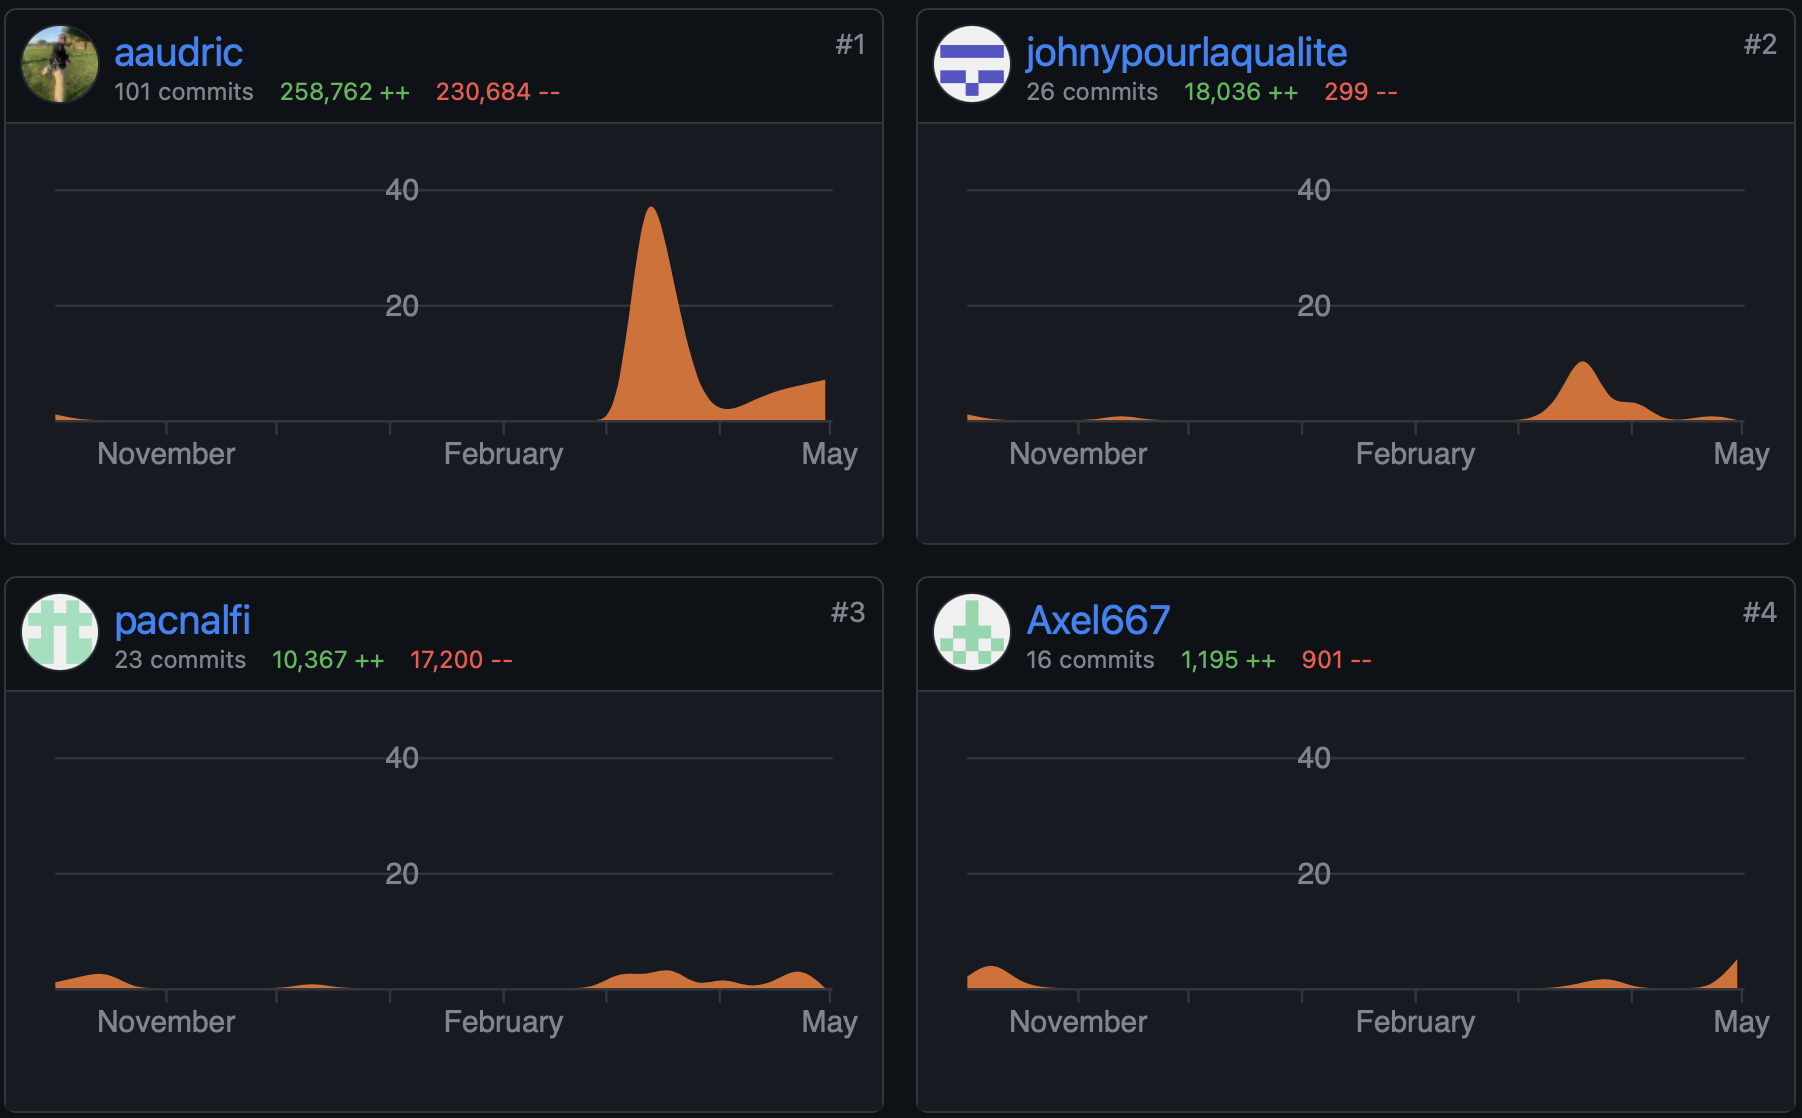
\includegraphics[width=1\textwidth]{images/contribution1.png}
        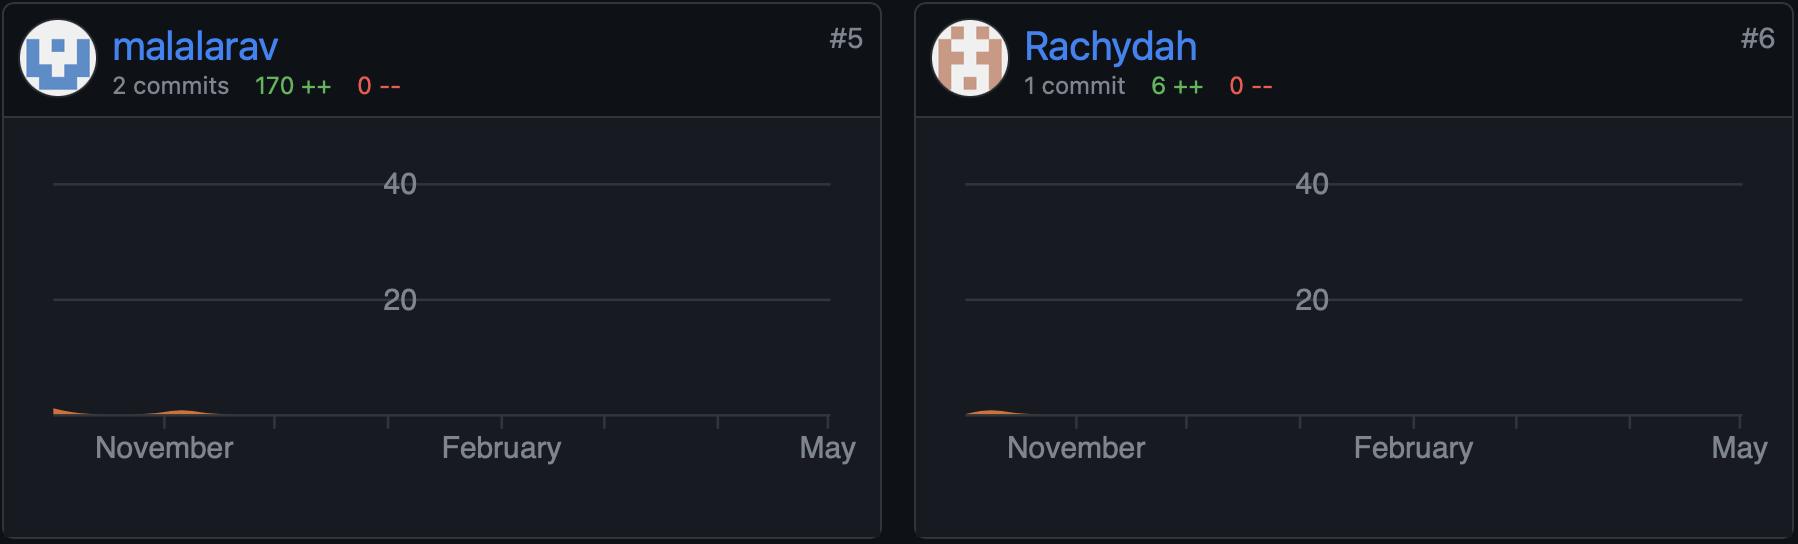
\includegraphics[width=1\textwidth]{images/contribution2.png}
\end{center}

\section{Difficultés rencontrées}
Nous n'avons pas rencontré de difficultés majeures pour la réalisation technique du projet, mise à part au niveau de la carte. En effet, cette tâche a pris plus de temps que prévu car nous avions des difficultés à afficher les données sur la carte. \\

Vers la fin du projet, il nous a aussi fallu prendre du recul sur le projet pour pouvoir nous mettre à la place de l'utilisateur et corriger certains détails au niveau du front-end pour le rendre plus ergonomique. \\

De plus, le passage en distanciel lors de la fermeture de l'université n'a pas contribué au bon développement du projet. Nous avons eu besoin d'un petit temps d'adaptation pour nous familiariser avec Git/GitHub qui ont été des outils indispensables pour l'avancement du projet en groupe. Cependant, nous avons su mettre en pratique les cours de gestion de projet du premier semestre. 

\section{Conclusions générales et perspectives}
Au niveau des perspectives, nous sommes globalement satisfaits du travail fourni. Cependant, le sujet que nous avons choisi est vaste. Nous aurions pu, par exemple, ajouter de nouveaux indicateurs ou encore prédire les données en lien avec l'économie et la santé des pays grâce à celles que nous possédons déjà. \\

De manière plus technique, nous aurions voulu rajouter la possibilité de modifier un article ou encore de mettre à disposition plus de données et sur une plus longue période, mais nous avons manqué de temps et n'avons pas trouvé plus de données. De plus, l'hébergement du site n'a pas pu être réalisé car nous n'avons pas trouvé de solution optimale. \\

Pour conclure, nous avons réussi à produire un site qui répond à tous les objectifs que nous nous étions fixés. La réalisation de ce projet a été exigeante, mais nous avons relevé ce défi. Nous avons pu mettre en pratique nos compétences en programmation web et nous sommes fiers du résultat.

\end{document}
